\documentclass[12pt]{article}
%\documentclass[border=0.1cm]{standalone}
\usepackage{wasysym}
\usepackage{phonenumbers}
\usepackage{marvosym }
\usepackage{xcolor}
\usepackage{comment}
\usepackage{pdfpages}
\usepackage[super]{nth}
\usepackage[paperwidth=8.5in,paperheight=11in,margin=0.5in]{geometry} 
\usepackage[UKenglish]{babel}
\usepackage[UKenglish]{isodate}% http://ctan.org/pkg/isodate
\usepackage{hyperref}
\hypersetup{
  colorlinks   = true, %Colours links instead of ugly boxes
  urlcolor     = black, %Colour for external hyperlinks
  linkcolor    = black, %Colour of internal links
  citecolor   = black %Colour of citations
}
\usepackage[activate={true,nocompatibility},final,tracking=true,kerning=true,spacing=true,factor=1100,stretch=10,shrink=10]{microtype}
\frenchspacing
\usepackage[nodayofweek,level]{datetime}
\usepackage{calc,url}
\newcounter{qz}\setcounter{qz}{0}
\newcommand{\qz}{%\
\setcounter{qz}{\value{qz}+1}
\textbf{In-class  \theqz} \,}

\newcounter{hw}\setcounter{hw}{0}
\newcommand{\hw}{%\
\setcounter{hw}{\value{hw}+1}
\textbf{HW \thehw}}

\newcounter{ex}\setcounter{ex}{0}
\newcommand{\ex}{%\
\setcounter{ex}{\value{ex}+1}
Exam \theex}

\usepackage[T1]{fontenc} 
\usepackage{fourier}
%\usepackage{tgschola} %to look retro
\newenvironment{mypar}[2]
  {\begin{list}{}%
    {\setlength\leftmargin{#1}
    \setlength\rightmargin{#2}}
    \item[]}
  {\end{list}}


\newcounter{wk}\setcounter{wk}{0}
\newcommand{\wk}{%\
\setcounter{wk}{\value{wk}+1}
\thewk \,\,}

\usepackage[nomessages]{fp}% http://ctan.org/pkg/fp


\usepackage{enumerate}
\usepackage{graphicx}

\usepackage{paralist}
\renewenvironment{description}[0]{\begin{compactdesc}}{\end{compactdesc}}

\newenvironment{alphalist}{
  \begin{enumerate}[(a)]
    \addtolength{\itemsep}{-0.5\itemsep}}
  {\end{enumerate}}
  \cleanlookdateon% Remove ordinal day reference
  \newcommand{\RomanNumeralCaps}[1]
      {\MakeUppercase{\romannumeral #1}}

\usepackage{xspace}
\makeatletter
\DeclareRobustCommand{\maybefakesc}[1]{%
  \ifnum\pdfstrcmp{\f@series}{\bfdefault}=\z@
    {\fontsize{\dimexpr0.8\dimexpr\f@size pt\relax}{0}\selectfont\uppercase{#1}}%
  \else
    \textsc{#1}%
  \fi
}
\newcommand\AM{\,\maybefakesc{am}\xspace}
\newcommand\PM{\,\maybefakesc{pm}\xspace}
\makeatother

 \newcommand{\coursename}{Advanced Calculus I}
\newcommand{\coursenumber}{MATH 460}
\newcommand{\sectionnumber}{01}
\newcommand{\term}{Fall }
\newcommand{\room}{Discovery Hall, room  386}
\newcommand{\meetingtime}{This class meets Monday, Wednesday, and Friday  from 
	9:05\AM -- 9:55\AM}
\newcommand{\officehours}{ Monday, Wednesday, and Friday 10:00\AM---11:00\AM,
    Tuesday and Thursday 9:30\AM---11:00\AM, and by appointment.}

    \newcommand{\finaldateandtime}{\printdate{13/12/\the\year} 8:00\AM{}---10:00 \AM}
\begin{document}
\cleanlookdateon% Remove ordinal day reference
\shortdate
\printyearoff
\large
\begin{center}
    \textbf{\coursename}  \\
    {\coursenumber---\sectionnumber} \\
     {\term \the\year} \\
\end{center}

\vskip0.25in
\normalsize


\begin{center}
\begin{description}
    \item[Instructor:] Barton Willis, PhD, Professor of Mathematics
    \item[Office:]  Discovery Hall, Room 368
    \item[\phone:]  \phonenumber[country=US]{3088658868}
    \item[\Email:]  \href{mailto:willisb@unk.edu}{willisb@unk.edu}
       % \item[Zoom:] 616 568 5706
    \item[Office Hours:] \officehours
  \end{description}
\end{center}



\subsubsection*{Important Dates}

\begin{mypar}{0.25in}{0.25in} 

  \textbf{First Homework due} \dotfill  \printdate{26/8/\the\year}  \\
  \textbf{Exam 1} \dotfill \printdate{15/9/\the\year}  \\
  \textbf{Exam 2} \dotfill  \printdate{13/10/\the\year} \\
  \textbf{Exam 3} \dotfill \printdate{10/11/\the\year} \\
  \textbf{Final exam} \dotfill  \finaldateandtime
\end{mypar}

\subsubsection*{Grading}

Your course grade will be based on twelve homework sets, three midterm exams, and a comprehensive 
final exam; specifically:
\FPeval{\hwpts}{round(20*12,0)}
\begin{mypar}{0.25in}{0.25in}
    \textbf{Weekly Homework:}  \emph{12 twenty point assignments}  \dotfill \hwpts\/ (total) \\
    \textbf{Mid-term exams 1, 2, and 3:} \emph{100 points each} \dotfill 300 (total)\\
    \textbf{Comprehensive Final exam} \dotfill 150 (total)
\end{mypar}
If we end the term with less than \hwpts\/ points for homework,  
your homework point total will be scaled to a total of. 

\FPeval{\points}{round(12*20+300+150,0)}

\FPeval{\F}{round(\points*0.6-1,0)}
\FPeval{\Dm}{round(\points*0.6,0)}
\FPeval{\D}{round(\points*0.633,0)}
\FPeval{\Dp}{round(\points*0.6667,0)}

\FPeval{\Cm}{round(\points*0.7,0)}
\FPeval{\C}{round(\points*0.733,0)}
\FPeval{\Cp}{round(\points*0.7667,0)}

\FPeval{\Bm}{round(\points*0.8,0)}
\FPeval{\B}{round(\points*0.833,0)}
\FPeval{\Bp}{round(\points*0.8667,0)}

\FPeval{\Am}{round(\points*0.9,0)}
\FPeval{\A}{round(\points*0.933,0)}
\FPeval{\Ap}{round(\points*0.99,0)}

The following table shows the \emph{minimum} number of points (out of \points) that
are required for each of the twelve letter grades D- through A+. For
example, a point total of \Bp\/  points will earn you a grade of B+,  and 
a point total of \Am\/ points will earn you a grade of A-. If you earn a point
total of \F\/  or less, you will a failing course grade.
 
 \vspace{0.1in}
     \begin{minipage}{5.5in}
  \centering 
\begin{mypar}{0.25in}{0.25in}
    \begin{minipage}{2.5in}
        D-  \dotfill \Dm \\
        D \dotfill \D \\
        D+ \dotfill \Dp \\
        C- \dotfill \Cm  \\
        C \dotfill \C \\
        C+ \dotfill \Cp 
        \end{minipage}
    \phantom{xxx}
    \begin{minipage}{2.5in}
        B- \dotfill \Bm \\
        B \dotfill  \B \\
        B+ \dotfill  \Bp\\
        A- \dotfill  \Am \\
        A \dotfill  \A \\
        A+ \dotfill  \Ap
    \end{minipage}
\end{mypar} 
\end{minipage}

\subsubsection*{Class meeting time and place}

\meetingtime in \room.

\subsubsection*{Course Resources}

Our textbook is \emph{An Introduction to Analysis}, \nth{2} edition, Waveland Press, Prospect Heights, Illinois, 2002 (ISBN 13: 978-1-57766-232-7) by James Kirkwood. The book by the same author and title, but published by PWS Publishing Company (Boston, 1995, ISBN 13:
0-534-94422-1) is identical.

 Some homework assignments for this course will need to be typeset. To do this, you will need to create a \emph{no cost} 
account on Overleaf (\url{https://www.overleaf.com/}).   For a  tutorial for using Overleaf, see \url{https://www.overleaf.com/tutorial}.



\subsubsection*{Course Calendar}

Generally, we'll adhere to the scheduled exam dates even if we are ahead or behind with coursework.  
When we are ahead or behind, the topics on the exams will be appropriately adjusted.  


\vspace{0.1in}
\noindent \textbf{Notices:}


\begin{alphalist}
   \item \emph{The three midterm exams will be given on  \textbf{Friday} of the week they are assigned.}
   
    \item Homework (labelled \textbf{HW}) will be due one minute before midnight on  Saturday of the week they are assigned.  

    \item The final exam will be given on \finaldateandtime.
    
\end{alphalist}

\vspace{0.1in}

\begin{center}
    \small
\begin{tabular}  {|l|l|l|l|l|}
\hline
\textbf{Week}  & \textbf{Week Starting} &  \textbf{Section(s)} & \textbf{Topic(s)} & \textbf{Assessments} \\
\hline \hline 
\wk    & \printdate{21/8/\the\year} &     & Logic, Proof methods, and Overleaf & \hw  \\
\wk    & \printdate{28/8/\the\year}   &  \S1.1 -- \S1.3  & Sets, Functions, Real numbers, Completeness   & \hw  \\
\wk    & \printdate{4/9/\the\year}&     \S2.1 -- \S2.2  & Sequences \& Subsequences    &  \hw \\
\wk    & \printdate{11/9/\the\year}&     \S2.1 -- \S2.2  & Sequences \& Subsequences    &    \textbf{\ex}   \\ \hline
\wk    & \printdate{18/9/\the\year}   &  \S2.3  & Bolzano-Weierstrass    &    \hw     \\ 
\wk    & \printdate{25/9/\the\year} &  \S3.1    &  Topology    &  \hw \\ 
\wk    & \printdate{2/10/\the\year}    & \S3.1  &   Topology  &    \hw  \\
\wk    & \printdate{9/10/\the\year}     & \S4.1  & Limits and Continuity & \textbf{\ex}  \\ \hline
\wk    & \printdate{16/10/\the\year}   & \S4.1  &  Limits and Continuity   &  \hw  \\ 
\wk    & \printdate{23/10/\the\year}      &   \S5.1 & Derivatives   & \hw \\ 
\wk    & \printdate{30/10/\the\year}   &   \S5.1 &  Derivatives   & \hw  \\
\wk    & \printdate{6/11/\the\year}  & \S5.2    & Some Mean Value Theorems   &  \textbf{\ex}    \\ \hline
\wk    & \printdate{13/11/\the\year} & \S6.1  & Some Mean Value Theorems   & \hw \\
\wk    & \printdate{20/11/\the\year}    &  \S6.2  & The Riemann Integral     &   \hw   \\
\wk    & \printdate{27/11/\the\year}   &   \S6.2    &  The Riemann Integral     &  \hw  \\ \hline
\wk   & \printdate{4/12/\the\year}     &  \S1.1--\S6.2   &   Catch up or review  &   \\  \hline
\wk   & \printdate{11/12/\the\year}     &    &    \hfill  & \textbf{ Final Exam}  \\  \hline  
\end{tabular}
\end{center}


\subsubsection* {Class Policies}

Unless an assessment is \emph{explicitly} stated to be a group project,  
\emph{all work you turn in for a grade must be your own.} If 
you need assistance completing a homework assignment, ask 
me for help. Each homework assignment you turn in for a grade must 
include the statement:

\begin{quote}
\fbox{I have neither given nor received unauthorized assistance on this assignment.}
\end{quote}
 If two assignments are so similar that only collaboration could explain their 
 similarities, both assignments will receive a grade of zero.  



Googling for answers, asking chatGPT to do your work, seeking help 
from the Learning Commons or other faculty members, or using a solution 
key from a previous terms (either from UNK or other universities) 
violates our class academic integrity policy.

If your homework involves concepts that are far more advanced than
our textbook and class work (for example, a Hausdorff space or the 
BLT theorem), I will take that as evidence of using unauthorized 
materials and you will earn a score of zero for that assessment.

Additional policies:
\begin{enumerate}

\item Generally, if you are ill, injured,  or absent for any reason (including 
athletics), you must turn in your in class work on time. Permission to
turn in work late must be made in advance, otherwise late in class work 
will count zero points.

\item During class time, please refrain from using electronic devices. If your 
device usage distracts your classmates, I will ask you to put it away. If it's my 
impression that you are often not paying attention in class, I reserve the right to 
decline to help you with homework assignments.



\item Using unauthorized materials or communication devices while taking a 
test will earn you a grade of zero on that assessment.  

\item It is essential and expected for you to attend class regularly. If you miss class, 
please ask a classmate for class notes. You may ask me for a copy 
of my class notes, but I might decline--it's unlikely my notes will be of any value 
you.

\item For examinations and in class assignments, show your work.  
\emph{No credit will be given for multistep problems without the necessary work. Your solution must contain enough detail
so that I am convinced that you could correctly solve any similar problem.} Also erase or clearly mark any work you want me to ignore; otherwise,
I'll grade it.  

\item The work you turn in for a grade must be \emph{accurate, 
complete, concise, neat}, and \emph{well-organized}.  
\emph{You will not earn full credit on work that falls short of 
these expectations.}

\item Class cancellations due to weather, illness, or other 
unplanned circumstances may require that we make  adjustments
to the course calendar, exam dates, or due dates for 
course assessments. 

\item I will \emph{decline} all requests for extra credit or for
redoing an assignment or examination to earn a higher grade.

\item For examinations, you may use a teacher provided quick reference sheet, 
but no other reference materials. You may also use a pencil, an eraser, 
and a scientific calculator. For examinations, your phone and all such
devices must be turned off and \emph{out of sight.} 

\item The final examination will be \emph{comprehensive} and it will be given 
during the  time scheduled by the University. Except for \emph{extraordinary circumstances}
you must take the exam at this time.
 
\item If you have questions about how your work has been graded, make an appointment with me immediately.

\item Please regularly check Canvas  to verify that your scores have 
been recorded correctly.  If I made a mistake in recording one of
your grades, I'll correct it provided you saved your paper.

\end{enumerate}

\subsubsection*{University Policies}

\paragraph*{Student Attendance Policy Statement}

Students are expected to attend all meetings of classes for which they are 
registered, including the first and last scheduled meetings and the final 
examination period. Instructors hold the right and responsibility to 
establish attendance policies for their courses. Each instructor must 
inform all classes at the beginning of each semester concerning their 
attendance policies.

Participation in official University activities, serious health concerns, 
personal emergencies, and religious observances are valid reasons for absence 
from classes. Students are responsible for informing their instructors prior 
to their absence(s) from class and for completing assignments missed during 
their absence(s). No adverse or prejudicial effects shall result to any student 
with a documented, excused absence.  

Questions may be directed to the Dean of Student Affairs office or to Student 
Health \& Counseling.

\paragraph{Academic Honesty Policy} Academic honesty is essential to the existence 
and integrity of an institution of higher education.  The responsibility for 
maintaining that integrity is shared by all members of the academic community.  
o further serve this end, the University of Nebraska at Kearney has a policy 
relating to academic integrity.   

\paragraph{Reporting Student Sexual Harassment, Sexual Violence or Sexual Assault}

Reporting allegations of rape, domestic violence, dating violence, sexual assault, 
sexual harassment, and stalking enables the University to promptly provide support 
to the impacted student(s), and to take appropriate action to prevent a recurrence 
of such sexual misconduct and protect the campus community. Confidentiality will 
be respected to the greatest degree possible. Any student who believes they may 
be the victim of sexual misconduct is encouraged to report to one or more of 
the following resources:

\begin{itemize}
  \item Local Domestic Violence, Sexual Assault Advocacy Agency 
      \phonenumber[country=US]{3082372599}

  \item Campus Police (or Security) \phonenumber[country=US]{3088658911}

  \item Title IX Coordinator \phonenumber[country=US]{3088658655}
\end{itemize}
Retaliation against the student making the report, whether by students or 
University employees, will not be tolerated.

\paragraph{Students with Disabilities} It is the policy of the University of Nebraska 
at Kearney to provide flexible and individualized reasonable accommodation 
to students with documented disabilities. To receive accommodation services 
for a disability, students must be registered with the UNK Disabilities Services 
for Students (DSS) office, 175 Memorial Student Affairs Building, 
\phonenumber[country=US]{3088658214} or by email 
\href{mailto:unkdso@unk.edu}{unkdso@unk.edu}  


\paragraph{Students Who are Pregnant} It is the policy of the University of Nebraska at Kearney to provide flexible and 
individualized reasonable accommodation to students who are pregnant. To receive 
accommodation services due to pregnancy, students must contact the 
Student Health office at \phonenumber[country=US]{3088658218}. The following links provide information 
for students and faculty regarding pregnancy rights: 

\begin{itemize}
\item \url{https://thepregnantscholar.org/title-ix-basics/} 

\item \url{https://nwlc.org/resource/faq-pregnant-and-parenting-college-graduate-students-rights/}

\end{itemize}

\paragraph{UNK Statement of Diversity \& Inclusion}

UNK stands in solidarity and unity with our students of color, our Latinx 
and international students, our LGBTQIA+ students and students from other 
marginalized groups in opposition to racism and prejudice in any form, 
wherever it may exist. It is the job of institutions of higher education, 
indeed their duty, to provide a haven for the safe and meaningful exchange of 
ideas and to support peaceful disagreement and discussion. In our classes, 
we strive to maintain a positive learning environment based upon open 
communication and mutual respect. UNK does not discriminate on the basis of 
race, color, national origin, age, religion, sex, gender, sexual orientation, 
disability or political affiliation. Respect for the diversity of our backgrounds 
and varied life experiences is essential to learning from our similarities as 
well as our differences. The following link provides resources and other 
information regarding D\&I: \url{https://www.unk.edu/about/equity-access-diversity.php}


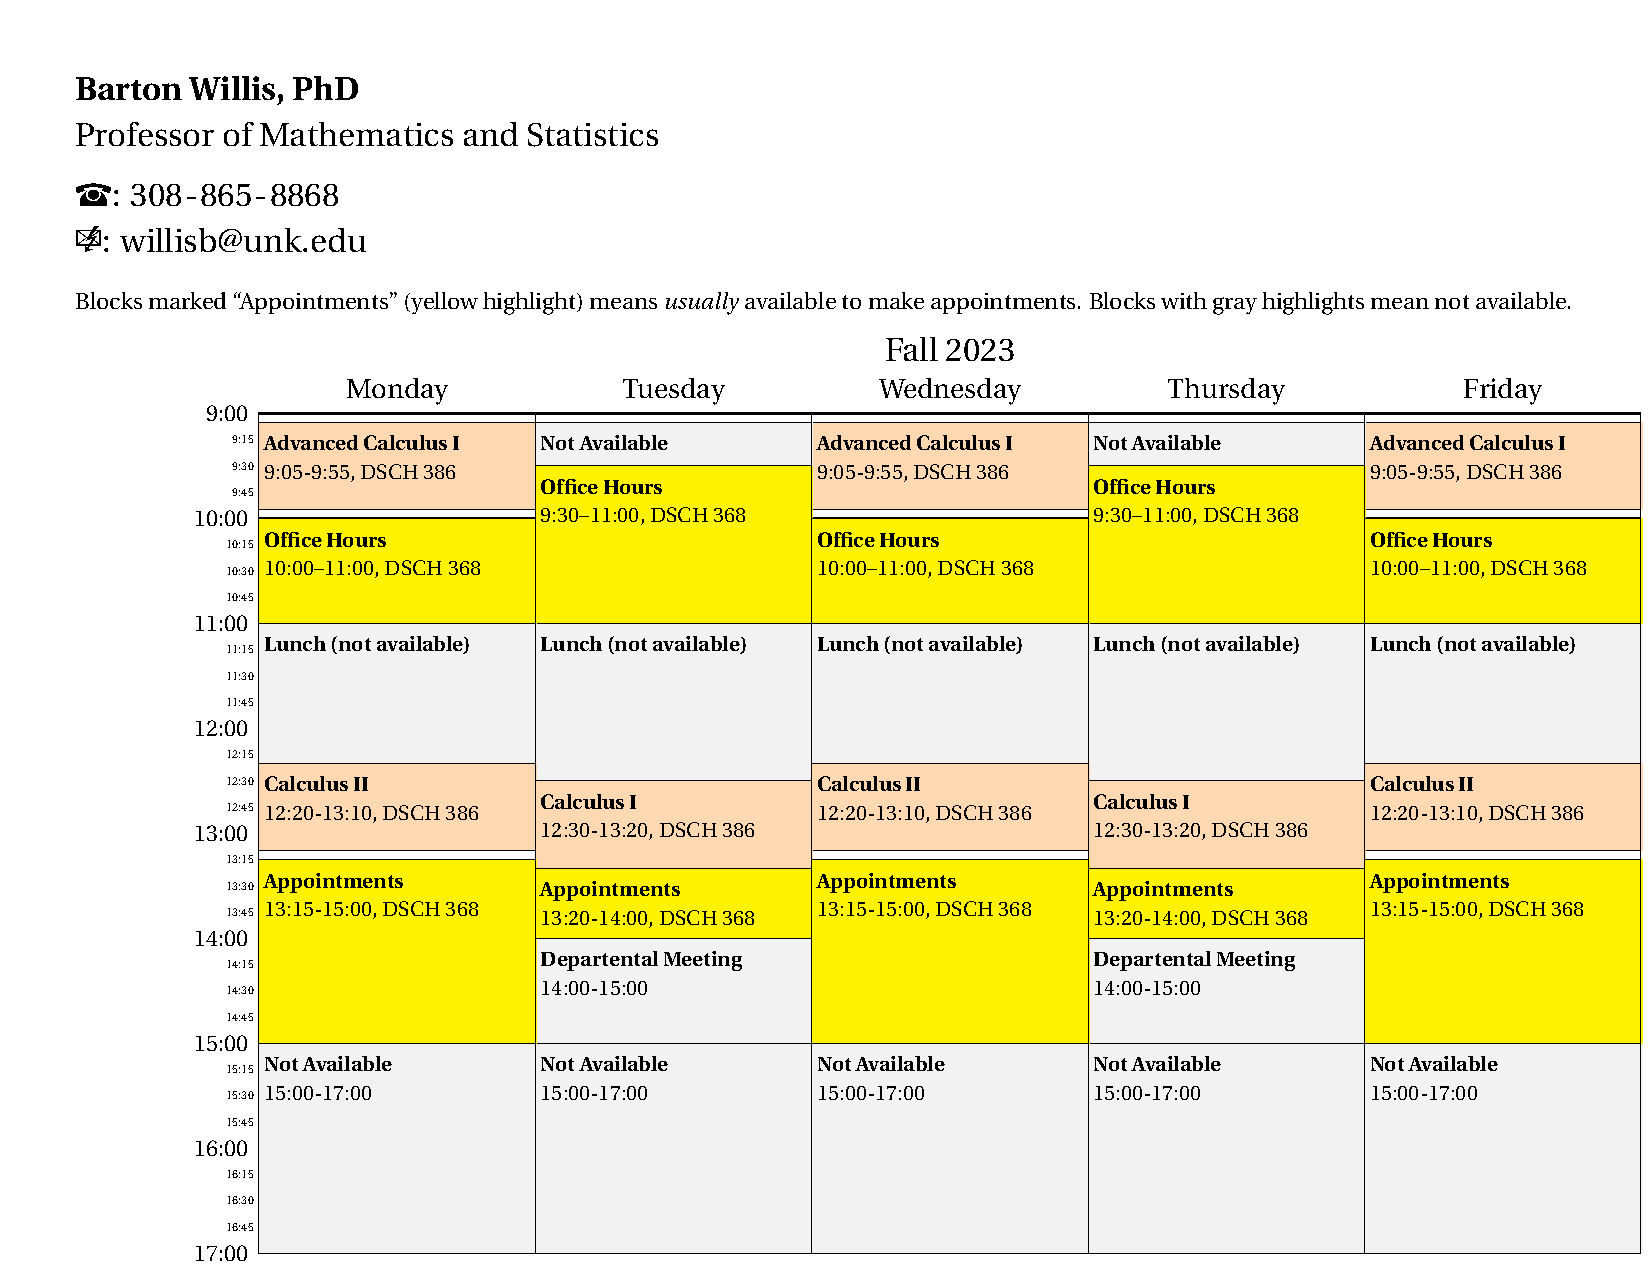
\includepdf[pages={1-},angle=90]{door_schedule.pdf}  
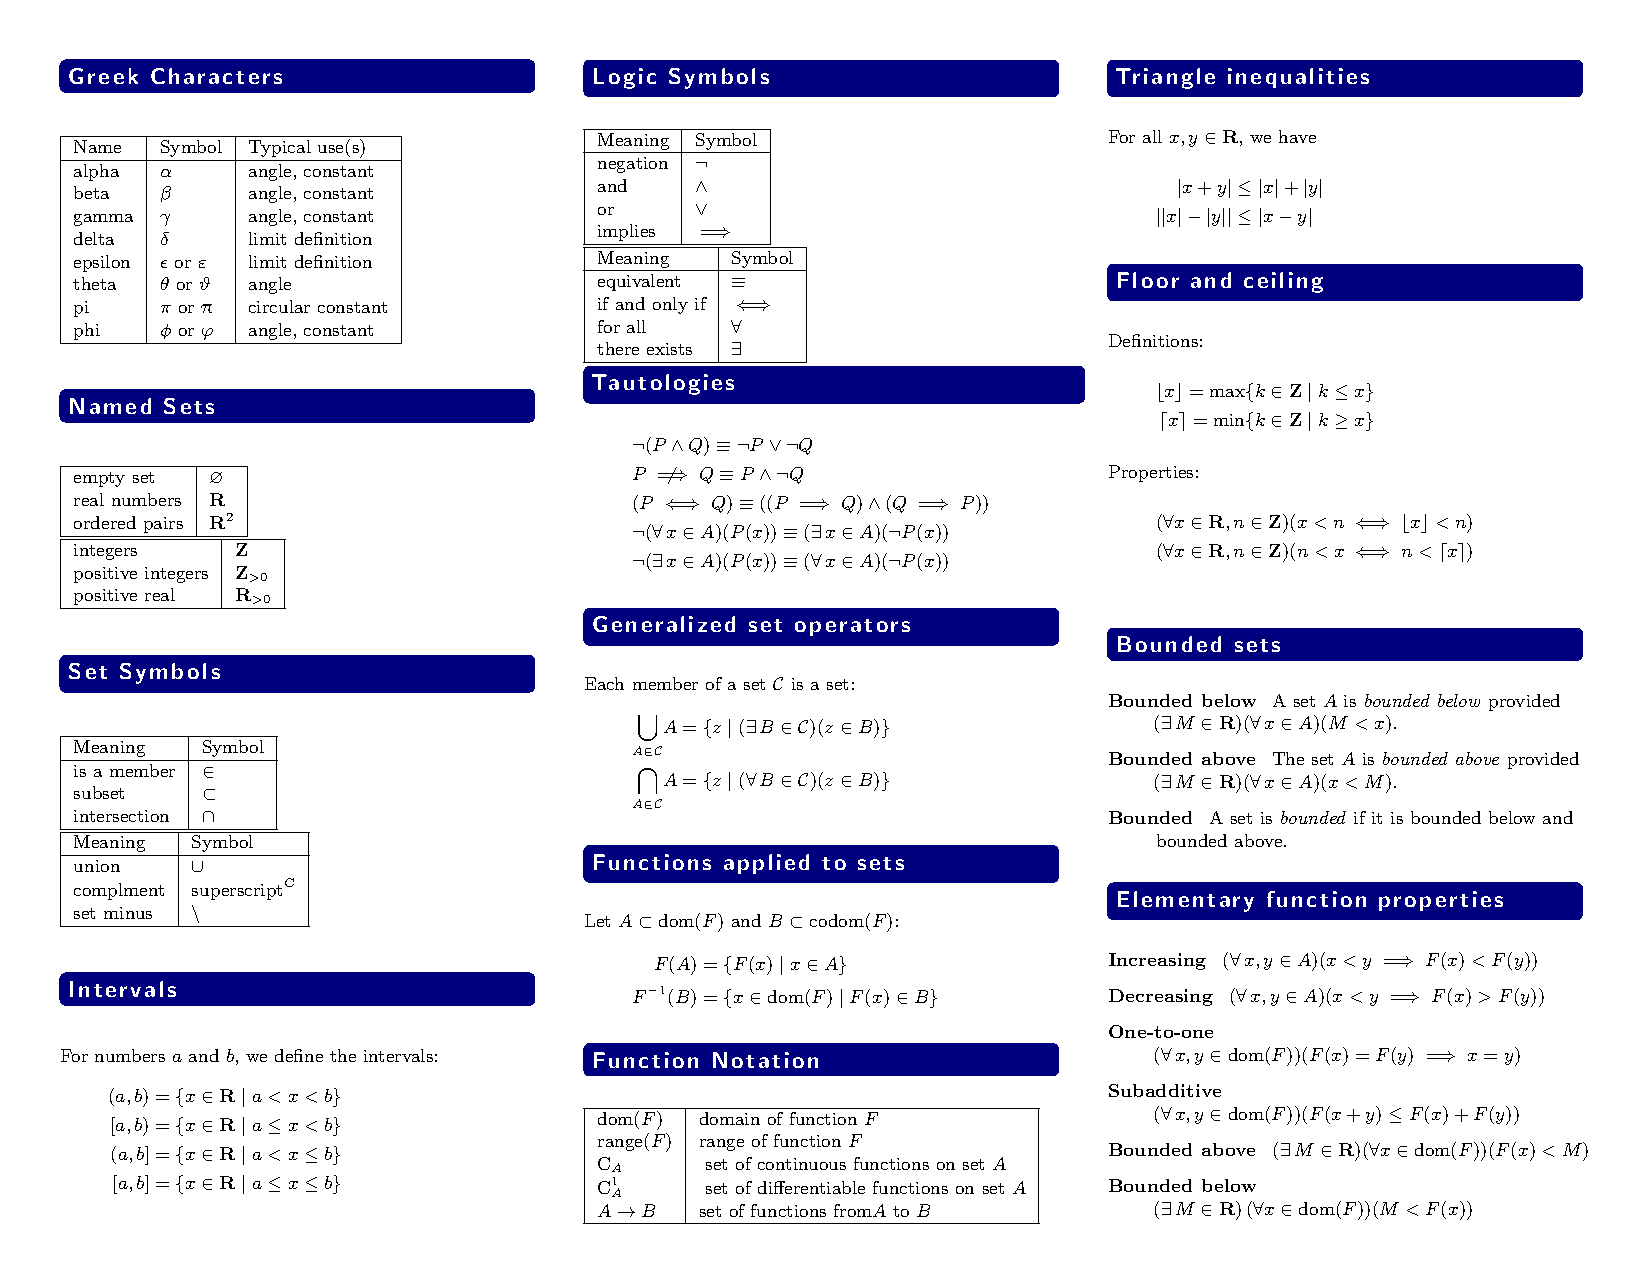
\includepdf[pages={1-},angle=90]{analysis-quick-reference.pdf} 
\end{document}

